\documentclass[a4paper,12pt,gray]{article}

\usepackage{préambule}
\usepackage{préambule-figures}
\usepackage{clipboard}
\usetikzlibrary{calc,positioning}

\renewcommand{\arraystretch}{1.2}

\begin{document}

\Copy{Cours}{
	\begin{cours}[Vocabulaire de la pyramide]
		\begin{center}
			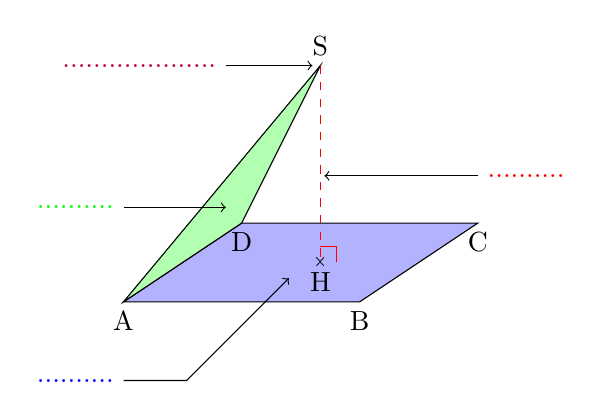
\begin{tikzpicture}
				\draw[fill=blue!30,draw=transparent] (0,0) -- ++(3,0) -- ++(1.5,1) -- ++(-3,0) -- cycle;
				\draw[fill=green!30,draw=transparent] (0,0) -- (1.5,1) -- (2.5,3) -- cycle;
				\draw[red,dashed] (2.5,3) -- ++(0,-2.5);
				\draw[red] (2.7,0.5) -- ++(0,0.2) -- ++(-0.2,0);
				\pyramide{3}{(1.5,1)}{(2.5,3)}

				% Points
				\node[below] at (0,0) {A};
				\node[below] at (3,0) {B};
				\node[below] at (4.5,1) {C};
				\node[below] at (1.5,1) {D};
				\node[above] at (2.5,3) {S};
				\node[below] at (2.5,0.5) {H};
				\node at (2.5,0.5) {{\tiny ×}};

				% Légendes
				\draw[->] (0,1.2) node[left] {{\color{green}..........}} -- ++(1.3,0);
				\draw[->] (1.3,3) node[left] {{\color{purple}....................}} -- ++(1.1,0);
				\draw[->] (0,-1) node[left] {{\color{blue}..........}} -- ++(0.8,0) -- ++(1.3,1.3);
				\draw[->] (4.5,1.6) node[right] {{\color{red}..........}} -- ++(-1.95,0);
			\end{tikzpicture}
		\end{center}
		\vspace{1em}

		La figure ci-dessus est une \textbf{............}.

		\begin{itemize}
			\item[\bullet] Sa \textbf{\color{blue}..........} est un polygone (triangle, quadrilatère, ...).
			\item[\bullet] Chaque \textbf{\color{green}................} est un triangle.
			\item[\bullet] La \textbf{\color{red}..........} de la pyramide est le segment [SH] : il part du point S, et est perpendiculaire à la base.
		\end{itemize}
	\end{cours}
}

\vspace{5em}
\Paste{Cours}

\end{document}